\chapter{Instance Segmentation}
\label{ch:lesson43}

Semantic segmentation (Chapter~\ref{ch:lesson42}) labels each pixel with a class, but it has no notion of \emph{how many} instances of each class there are --- two touching instances are just labeled as one connected blob of pixels. \textbf{Instance segmentation} answers the harder question: which pixels belong to \emph{this specific} object, as opposed to some other object of the same class. This chapter augments Chapter~\ref{ch:lesson42}'s segmentation network directly to solve it, with an idea that traces straight back to Chapter~\ref{ch:lesson12}'s Hough transform: instead of only classifying pixels, have the network also predict, for every foreground pixel, a vote for where its object's center is --- then cluster the votes to recover individual instances.

\section{Overlapping instances}

Two circles per scene, deliberately placed close enough to touch or overlap. Ground truth includes both a semantic mask (0=background, 1=circle) and an \emph{instance} mask (0=background, 1=first circle, 2=second circle), as shown in Figure~\ref{fig:l43-1}.

\begin{figure}[h]
\centering
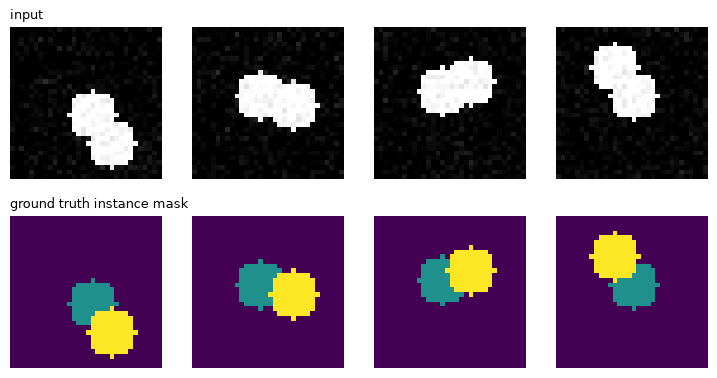
\includegraphics[width=0.9\textwidth]{figures/lesson43_fig01.png}
\caption{Input images (top row) and their ground-truth instance masks (bottom row).}
\label{fig:l43-1}
\end{figure}

\section{Augmenting the network with an instance head}

Take Chapter~\ref{ch:lesson42}'s exact U-Net architecture and give it a second output head alongside the semantic head: for every foreground pixel, predict a $(dx,dy)$ offset pointing toward its own instance's center. The semantic head still does the same job as Chapter~\ref{ch:lesson42} (background vs.\ circle); the new offset head is what turns plain segmentation into \emph{instance} segmentation.

\begin{lstlisting}
class InstanceNet(nn.Module):
    """U-Net, with a second head: per-pixel offset-to-center regression"""
    def forward(self, x):
        f1 = self.enc1(x)
        f2 = self.enc2(self.pool(f1))
        d1 = self.dec1(torch.cat([self.up(f2), f1], dim=1))
        return self.sem_head(d1), self.offset_head(d1)
\end{lstlisting}

Trained for 300 epochs with a weighted sum of cross-entropy (semantic head) and MSE (offset head, masked to foreground pixels only): semantic pixel accuracy $100.0\%$.

\section{Recovering instances: vote for the center, then cluster (Hough, again)}

The offset head above was trained to predict, for every foreground pixel, an offset pointing toward \emph{its own instance's} center --- supervised directly from the ground-truth instance masks. Each foreground pixel casts one vote (its predicted center location) into an accumulator, exactly like Chapter~\ref{ch:lesson12}'s Hough line/circle voting. Because every pixel belonging to the same circle votes for approximately the same point, the accumulator forms one tight cluster of votes per instance, however tangled the pixels themselves are. Finding instances becomes: find the vote clusters, then assign each pixel to its nearest cluster.

\begin{lstlisting}
# greedily take the highest-voted peak, suppress its neighborhood, repeat
# (the same non-max-suppression idea as Chapter 40's detection boxes)
for _ in range(6):
    idx = np.unravel_index(votes_work.argmax(), votes_work.shape)
    if votes_work[idx] < vote_thresh:
        break
    peaks.append((idx[1], idx[0]))
    votes_work[y0:y1, x0:x1] = 0  # suppress the neighborhood around this peak
\end{lstlisting}

Offset-voting recovers the correct instance count in $44/45$ test scenes ($97.8\%$), shown in Figure~\ref{fig:l43-2}.

\begin{figure}[h]
\centering
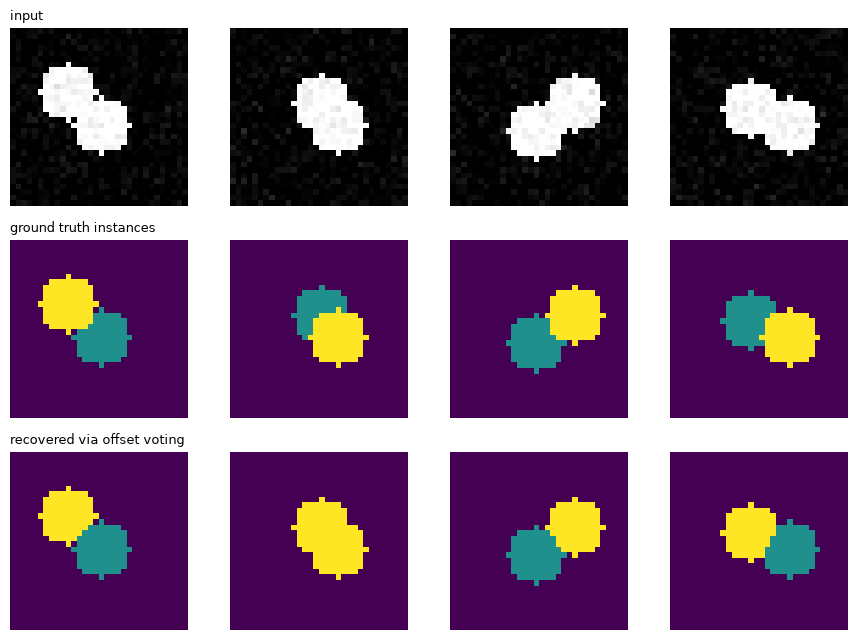
\includegraphics[width=0.9\textwidth]{figures/lesson43_fig02.png}
\caption{Input, ground-truth instances, and instances recovered via offset voting, for four test scenes.}
\label{fig:l43-2}
\end{figure}

\section{Mask R-CNN: Faster R-CNN plus a mask branch}

The offset-voting approach above is one family of instance segmentation methods (related to techniques sometimes called ``instance embedding'' or center-voting). The other dominant approach, \textbf{Mask R-CNN} (\citelink{he2017maskrcnn}{He et al., 2017}), does not start from scratch --- it is \textbf{Faster R-CNN} (Chapter~\ref{ch:lesson41}) with one new piece bolted on. The region proposal network, the per-box classifier, and the per-box coordinate refinement are all unchanged. Mask R-CNN just adds a third, parallel branch on every detected box: alongside the existing class label and refined box coordinates, a small fully-convolutional head predicts a binary mask \emph{within that box}. Detection already solves ``how many objects, and roughly where'' via region proposals and NMS; the mask branch adds ``and here's this one's exact silhouette'' --- exactly the piece built and tested in isolation below.

One more change was needed to make that mask branch actually work well. Faster R-CNN extracts a fixed-size feature grid for each proposed box by snapping (quantizing) the box's coordinates to the nearest feature-map cell --- a step called RoIPool. That rounding barely affects classifying a box or nudging its coordinates by a few pixels, but it visibly misaligns a per-pixel mask against the object it is supposed to outline. Mask R-CNN replaces RoIPool with \textbf{RoIAlign}, which reads features via bilinear interpolation instead of rounding to the nearest cell, so the extracted features --- and therefore the predicted mask --- stay aligned with the actual box coordinates. This is a small change to the detector, but it is the specific fix that makes pixel-accurate masks possible.

Putting Chapters~\ref{ch:lesson36}, \ref{ch:lesson40}, \ref{ch:lesson41}, and this chapter together: \textbf{classification} (Chapter~\ref{ch:lesson36}) gives one label for the whole image, \textbf{semantic segmentation} (Chapter~\ref{ch:lesson42}) gives one label per pixel with no notion of separate objects of the same class, and \textbf{instance segmentation} (this chapter) adds a distinct identity per object --- ``background,'' ``circle \#1,'' ``circle \#2,'' not just ``background,'' ``circle.'' A fourth term, \textbf{panoptic segmentation}, unifies the last two: every pixel gets both a semantic class and, for countable ``thing'' classes like circles or cars, an instance ID --- while uncountable ``stuff'' classes like sky or road are labeled semantically only, since instance identity doesn't make sense for them.

\section{A mask head}

Detection (Chapter~\ref{ch:lesson41}) and per-instance masking are two separate, already-solved pieces at this point --- the only genuinely new ingredient Mask R-CNN adds is the \textbf{mask head}: a small network that looks \emph{only} inside one proposed box and predicts a binary mask for the single object that box was proposed for, ignoring anything else visible in the crop.

Build that piece in isolation. Take the ground-truth box around each instance's true center (assume localization is already solved, so only the new mask-head idea is under test), crop a fixed $14\times14$ window there, and train a tiny fully-convolutional head to predict which pixels in that crop belong to \emph{this} instance --- not to any neighboring circle that happens to also be visible in the same crop. This produces $510$ training crops and $90$ test crops, each $14\times14$.

\begin{lstlisting}
class MaskHead(nn.Module):
    def __init__(self):
        super().__init__()
        self.net = nn.Sequential(
            nn.Conv2d(1, 16, 3, padding=1), nn.ReLU(),
            nn.Conv2d(16, 16, 3, padding=1), nn.ReLU(),
            nn.Conv2d(16, 1, 1),  # per-pixel mask logit, full crop resolution throughout
        )
\end{lstlisting}

Trained for 300 epochs with binary cross-entropy: mask-head IoU (per-instance) $0.844$, versus a naive ``everything foreground in the crop'' baseline IoU of $0.687$ (Figure~\ref{fig:l43-3}).

\begin{figure}[h]
\centering
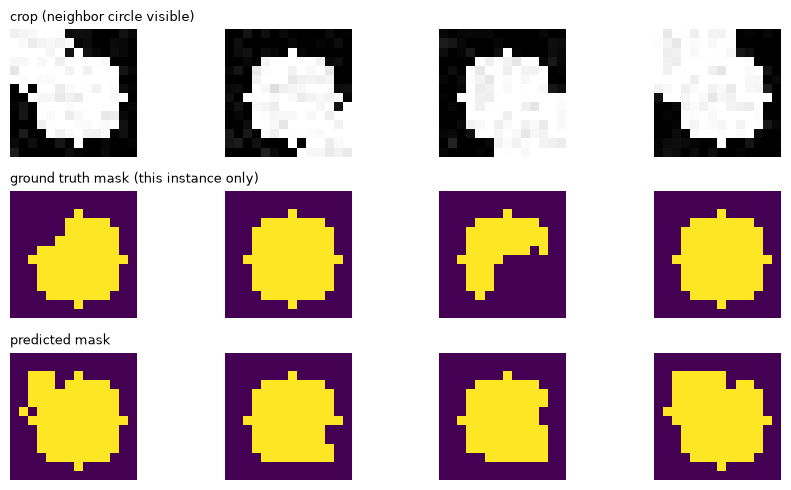
\includegraphics[width=0.9\textwidth]{figures/lesson43_fig03.png}
\caption{Crops (with a neighboring circle visible), ground-truth per-instance masks, and predicted masks.}
\label{fig:l43-3}
\end{figure}

Because this dataset's circles are generated close enough to always touch or overlap, \emph{every single test crop} contains visible pixels from the neighboring circle --- there is no ``easy'' case here to inflate the numbers. The per-instance mask head still reaches a respectably high IoU against the true single-instance mask, clearly ahead of the naive baseline that just marks every foreground pixel in the crop as belonging to ``the'' object (which is systematically wrong whenever a neighbor intrudes --- the same problem that motivated giving the network an instance-center head in the first place, just replayed at crop scale). The mask head doesn't need to solve ``where are the circles'' --- the box already answered that --- it only has to learn ``given that this box was proposed for one specific circle, which pixels are that circle's, and not its neighbor's.'' That's a strictly easier, more local question, which is exactly why Mask R-CNN's mask branch can be small and fast: a good box already does most of the work.

This also clarifies why Mask R-CNN and this chapter's offset-voting approach rarely fail the same way. Offset-voting can mis-cluster votes when two instances' centers are close enough that their accumulator peaks blur together. Mask R-CNN instead depends on the upstream detector proposing a correct box for every instance in the first place --- miss a box, and that instance's mask is never even attempted, no matter how good the mask head is.

\section{In practice: Mask R-CNN on a real photo}

The mask head above proves the idea works once localization is solved for free (ground-truth box centers). Here is the same idea, fully assembled and pretrained: a real \textbf{Mask R-CNN} (\code{torchvision.models.detection.maskrcnn\_resnet50\_fpn}, trained on COCO) run end to end --- detection and mask head both included, nothing given away --- on a photo with exactly the kind of touching, same-class instances this chapter has been building toward: the same Apollo 11 crew photo from Chapters~\ref{ch:lesson40}--\ref{ch:lesson41}.

Above $80\%$ confidence: 4 instances --- three \code{person} detections (each $\geq99.8\%$) and one spurious \code{clock} detection ($83.6\%$), shown in Figure~\ref{fig:l43-4}.

\begin{figure}[h]
\centering
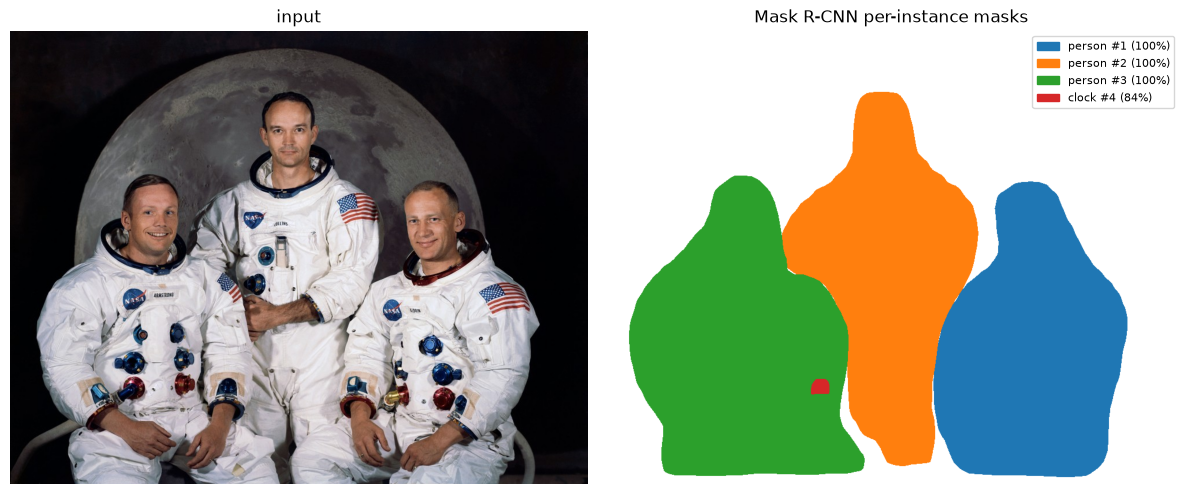
\includegraphics[width=0.95\textwidth]{figures/lesson43_fig04.png}
\caption{Real Mask R-CNN per-instance masks. \attrib{Image source: NASA (public domain), via Wikimedia Commons.}}
\label{fig:l43-4}
\end{figure}

The three astronauts are shoulder-to-shoulder, touching along multiple arm and torso boundaries, and belong to the exact same COCO class (\code{person}) --- precisely the case where a semantic mask would merge them into one undifferentiated blob. Mask R-CNN separates them cleanly into three distinct instances anyway, because its detector proposes three separate boxes first (one per astronaut) and the mask head only looks inside a single box at a time, exactly like the mask head above. The fourth, spurious detection is a small \code{clock} mask on the left astronaut's wrist --- the round, mirrored cuff-mounted checklist on Armstrong's arm, misread as a clock face.

\subsection*{Exercises}
\begin{enumerate}
  \item Reduce \code{dist} in \code{make\_scene} from the range $(6,9)$ to $(2,5)$, making the circles overlap much more heavily (centers closer together). Does the offset-voting method's instance-count accuracy hold up, or does it start failing too --- and if so, what does the failure look like (merged instances, split instances, or something else)?
  \item The clustering here uses \code{peak\_dist=4} for non-max suppression on the vote accumulator. Try \code{peak\_dist=8}. Does accuracy improve, get worse, or become sensitive to exactly how close two true circle centers happen to be in a given scene?
  \item This chapter only ever has 2 circles per scene. Extend \code{make\_scene} to place a random number of circles (1 to 4). Does the offset-voting approach's instance count accuracy hold up as the true number of instances grows?
  \item The mask head above was trained and evaluated using the \emph{ground-truth} box center, sidestepping detection entirely. Perturb each crop's center by a few random pixels before cropping (simulating an imperfect detector) and rerun. How much does mask IoU degrade as the box gets less accurately centered?
\end{enumerate}

\vfill
\fullcode{lesson43}{lesson43_instance_segmentation}
